\documentclass[USenglish,oneside,twocolumn]{article}
\usepackage[utf8]{inputenc}
\usepackage[big]{dgruyter_NEW}

\usepackage[backend=biber,natbib=false]{biblatex}
\addbibresource{references.bib}
  
\begin{document}
\title{\huge Smart Climate and Air Quality Control Systems}

\runningtitle{Running title}
\journalname{Internet of Things Projects}
\startpage{1}

\begin{abstract}
    {Smart climate and air quality control systems are transforming indoor environments by using IoT, advanced sensors, and automation to optimize temperature, humidity, and air quality. These systems monitor pollutants like CO and enhance energy efficiency, creating healthier and more sustainable spaces. This short paper examines a modular IoT-enabled system powered by the PineCone1 microcontroller, which uses sensors like DHT22 and MQ-2. Features include autonomous operation, secure data transmission via MQTT, and user-friendly interfaces. Applications in residential, healthcare, and urban settings demonstrate scalability and adaptability, while emerging technologies like machine learning and smart city integration can be used to further improve their effectiveness. Despite challenges such as sensor calibration and data privacy, these systems offer significant potential for health, energy savings, and sustainability.}
\end{abstract}

\maketitle

\section{Introduction}
Smart homes are becoming increasingly popular as technology advances, offering convenience and enhanced living experiences. However, these luxuries often come with a hefty price tag due to the sophisticated and complex technology they require, the cost of installation, and the need for regular maintenance.\cite{alam_2024_ambientiq}\cite{barot_2020_towards} One essential component of smart homes is Air Quality monitoring technology, which has been widely used across industries such as food processing, healthcare and pharmaceuticals, and smart cities and urban development, etc. In the context of smart homes, temperature sensors play a pivotal role in smart climate and air quality control systems. These sensors are reliable, accurate, and versatile, providing several advantages such as reducing energy costs, improving appliance safety, and increasing heating or cooling efficiency depending on the circumstances. By integrating temperature monitoring into smart home setups,\cite{barot_2020_air} homeowners can monitor energy consumption, regulate temperature effectively, and enhance overall energy efficiency. Amidst an energy procurement crisis, especially in regions like Europe, such systems have become increasingly critical. Smart climate control systems equipped with temperature sensors can optimize the operation of gas-based heaters, enabling users to save significant energy costs while reducing emissions that harm the environment. These systems ensure heaters operate only when necessary, preventing overuse and maintaining desired temperatures, thereby conserving energy and resources. Modern smart systems go beyond temperature regulation by integrating air quality control features to detect and address harmful gases like CO2.\cite{adhiwibowo_2020_temperature} By automating ventilation and providing real-time alerts, these systems promote healthier indoor environments while dynamically adjusting heating, cooling, and ventilation based on real-time data. Advanced sensors optimize temperature, humidity, and air quality, seamlessly integrating with home automation to enhance energy efficiency and sustainability. This dual focus on climate and air quality creates more sustainable, efficient, and eco-friendly living spaces. These IoT-enabled technologies are transforming indoor environmental management, making homes smarter, greener, and more comfortable while ensuring safety and health. The system is versatile, serving homes, schools, and healthcare facilities by maintaining ideal conditions for comfort, learning, and patient care. Its scalability and adaptability make it a key component in smart city development, enhancing urban living standards while supporting climate change mitigation and resource efficiency.\cite{fisk_2015_review}

\section{Literature Review}
Smart homes equipped with indoor air quality (IAQ) management systems represent a transformative approach to creating healthier and more sustainable living environments. By integrating interconnected sensors, automation, and real-time analytics, these systems optimize indoor conditions such as temperature, humidity, and air quality while addressing pollutants like carbon dioxide (CO2). Originally centered on energy efficiency, modern smart home technologies now prioritize IAQ management to mitigate health risks, such as respiratory issues and cognitive impairments, which are aggravated by poor air quality and environmental pollution. Studies have highlighted the effectiveness of these systems, with Fisk\cite{ghoneim_2019_towards} emphasizing their role in mitigating health risks linked to climate change, particularly for vulnerable populations. Similarly, Wallner et\cite{wallner_2017_health} al. demonstrated that mechanical ventilation systems in energy-efficient homes maintain better IAQ compared to naturally ventilated homes, especially in urban settings where exposure to outdoor pollutants is higher. Additionally, Kumar et al.\cite{schieweck_2018_smart} showed how demand-driven, data-responsive ventilation systems in smart homes not only improve IAQ but also significantly reduce energy consumption. Recent advancements in this field include IoT-enabled multi-sensor networks, which provide affordable and accessible real-time monitoring of IAQ metrics, and predictive analytics powered by machine learning, which can anticipate air quality fluctuations and adjust climate controls proactively. These technologies now extend their applications beyond residential spaces to include schools, where they promote healthier learning environments, and healthcare facilities, where they support infection control and enhance patient care. The integration of IAQ systems with Ambient Assisted Living (AAL)\cite{das_2022_how} solutions has also expanded their scope to include health tracking for elderly populations, showcasing their potential in specialized healthcare contexts. Furthermore, smartphone integration allows users to remotely monitor IAQ and receive alerts, offering greater convenience and control.

Despite these advancements, challenges remain. A significant research gap lies in the lack of standardized protocols for IAQ sensors, resulting in inconsistent data accuracy across different environments. Moreover, the integration of IAQ systems with broader urban environmental monitoring frameworks is still underexplored, despite its relevance in densely populated areas where outdoor air quality concerns are prominent. While existing studies underscore the short-term health benefits of improved IAQ, there is a need for longitudinal research to assess the sustained impacts, particularly for children, the elderly, and other vulnerable groups. Additionally, debates persist over the extent of automation versus user control in these systems, with some users preferring manual adjustments despite the proven benefits of automated optimization. Data privacy and security also remain critical concerns, as IAQ systems collect detailed information about home environments and occupant behaviors, necessitating robust safeguards against unauthorized access.\cite{salthammer_2011_critical} In conclusion, smart home technologies integrated with IAQ management systems hold immense potential to revolutionize indoor climate control and promote healthier, more sustainable living spaces. However, addressing challenges like sensor standardization, urban integration, and privacy concerns is crucial for unlocking their full potential. These systems not only enhance individual health and well-being but also contribute to broader goals like climate change mitigation, urban sustainability, and the development of smart cities. By advancing research and addressing current limitations, smart IAQ systems can play a pivotal role in shaping a future where indoor environments are healthier, safer, and more efficient.

In another research paper we found that The integration of Internet of Things (IoT) technologies has revolutionized traditional environmental monitoring by giving rise to advanced smart climate and air quality control systems, which autonomously regulate indoor environments to enhance occupant comfort, health, and safety. These systems rely on IoT-enabled sensors and microcontrollers to monitor and adjust critical parameters such as temperature, humidity, and pollutant levels in real-time, ensuring a balanced and optimized indoor atmosphere. For example, systems like the Smart Climate and Air Quality Control System use a network of sensors, including the DHT22 for humidity and temperature monitoring, alongside CO2 and CO gas sensors for detecting air pollutants, providing detailed environmental data that is essential for maintaining healthy conditions. The core objectives of these systems include improving air quality, maintaining thermal comfort, and enhancing energy efficiency by making adjustments only when necessary. Automation plays a central role in these systems, using real-time data processing to activate devices such as air purifiers, heaters, and humidifiers, ensuring optimal environmental conditions with minimal energy consumption. Additionally, user interaction is facilitated through intuitive interfaces like smartphone apps, allowing users to monitor and adjust system settings, view real-time environmental data, and receive alerts. This level of user engagement ensures that the system is customized to meet individual needs, improving user satisfaction. However, despite the benefits, IoT-based climate control systems face several challenges. Sensor calibration and data accuracy remain significant concerns, as low-cost sensors can experience calibration drift, leading to inaccuracies in pollutant level measurements. Regular recalibration is needed to maintain system performance, especially in applications where precise monitoring of pollutants is critical. Moreover, power management is a key issue in battery-operated systems, necessitating the development of energy-efficient protocols and optimized sampling rates to extend system longevity. Looking ahead, emerging trends in IoT-based climate control systems include the use of machine learning algorithms to predict and adjust climate parameters proactively, based on historical data and environmental conditions. These advancements can enhance system responsiveness to fluctuations in air quality, providing more effective climate management. Furthermore, integrating these systems into smart city infrastructures offers vast potential for community-wide health and environmental monitoring. By collecting and analyzing data on both indoor and outdoor air quality, these systems can support urban planning, public health initiatives, and environmental policy-making. In conclusion, IoT-based smart climate and air quality control systems present a transformative solution for creating healthier and more sustainable indoor environments. With ongoing advancements in sensor accuracy, machine learning, and energy-efficient technologies, these systems are poised to play a crucial role in improving indoor air quality, reducing energy consumption, and promoting overall well-being. Future developments in sensor reliability, smart city integration, and energy efficiency will continue to expand the impact of these systems, enabling smarter, healthier, and more sustainable urban living spaces.

\section{Research Questions}
\begin{enumerate}
\item How can IoT technology enhance real-time monitoring and control of indoor conditions, specifically temperature, humidity, and air quality\cite{schieweck_2018_smart} 
\item What configurations and placements of sensors are most effective for accurate, continuous data collection in indoor environments? 
\item How efficiently does the PineCone1 microcontroller process data from multiple environmental sensors to support real-time system responses? 
\item How does the MQTT protocol contribute to low-latency, secure data transmission within this IoT-based system?
\item Can combining threshold-based algorithms with machine learning improve climate control, optimizing comfort and energy efficiency in smart homes? 
\item What impact does user customization, such as setting environmental thresholds, have on user satisfaction and system adaptability? 
\item How critical is ongoing sensor calibration to maintaining the accuracy and reliability of environmental data over time? 
\item How effectively does the system's modular design support scalability for additional sensors or devices? 
\item What cybersecurity risks exist for IoT-based climate control systems, and how can these be minimized? 
\item How does real-time data visualization on mobile and or web platforms improve user interaction and control over indoor environmental conditions?
\end{enumerate}

\section{Project Background}
The Smart Climate and Air Quality Control System leverages the Internet of Things (IoT) to autonomously monitor and manage indoor environmental conditions, ensuring safe and comfortable levels of temperature, humidity, and air quality. With increasing concerns over indoor environmental quality, this system addresses common issues such as CO2 accumulation, fluctuating temperature, and humidity levels. It aims to create healthier, more energy-efficient living and working environments by utilizing advanced sensors and real-time data processing. This project explores the integration of IoT technologies to provide a scalable solution for various settings, including residential, healthcare, and urban environments.

\section{Methodology}
A qualitative approach was followed to develop the system, starting with an analysis of existing research to understand current challenges, outcomes, and technological gaps. The system design builds upon this analysis, focusing on overcoming challenges to improve functionality. The methodology involves gathering data from research papers, project reports, and other available resources, which are mostly accessible online. Key to the system's design is a modular IoT-based architecture that uses various sensors and automation to autonomously manage indoor conditions. The core of the system is the PineCone1 microcontroller, which interfaces with a network of sensors. Data is collected in real time, processed, and then acted upon through automated responses. The system also uses secure communication via TCP/IP, ensuring that sensitive data is transmitted safely and efficiently. Programming is done using C. C is employed for low-level hardware control of the PineCone1 microcontroller, while C is used for higher-level backend processing and interface management. This ensures seamless integration between hardware and software. The system operates using threshold-based algorithms that control environmental conditions, such as activating the heater when the temperature drops below a set point or increasing ventilation when CO levels rise. Users interact with the system via secure, encrypted web or mobile interfaces, where they can monitor real-time data, adjust thresholds, and receive alerts. Testing involves multiple stages, including component, integration, and user testing. Sensor and device placement, along with regular maintenance and recalibration, ensure optimal performance and long-term reliability. The system's design allows for scalability, enabling the addition of more sensors or devices to adapt to different environments and improve functionality.

\section{Hardware Setup}
The hardware setup for the Smart Climate and Air Quality Control System consists of several key components: PineCone1 Microcontroller: This is the heart of the system, responsible for processing data from the sensors and controlling the connected devices. It communicates with all the components through digital or analog pins. DHT22 Sensor: This sensor measures temperature and humidity levels. It uses a single-bus communication protocol to send data to the microcontroller.\cite{dutta_2016_airsense} MQ-2 Gas Sensor: Used to detect various pollutants such as CO and Butane. It provides real-time data about the concentration of gases in the environment.\cite{adhiwibowo_2020_temperature}

2-channel-relay Module (12V): This module allows the microcontroller to control external devices, such as fans or heaters, by switching on or off depending on the environmental conditions. Arctic P12 Fan: A fan used to regulate air circulation within the indoor space, ensuring better air quality and comfort. PTC 100W 12V Heater: This device helps maintain the desired temperature by heating the indoor space when necessary. Wi-Fi Module: For secure data transmission via the MQTT protocol, ensuring efficient and responsive communication between the system and remote devices (mobile or web interface). The sensors and devices are strategically placed in the environment for optimal data collection and management. The modular design allows for easy integration of additional components, providing flexibility to expand the system's capabilities. In summary, the hardware setup forms a robust and flexible foundation for managing indoor environmental conditions. The system's combination of sensors, actuators, and secure communication protocols ensures that it can autonomously control temperature, humidity, and air quality, offering a sustainable solution for automated indoor climate management.

\begin{figure}[h] 
    \centering
    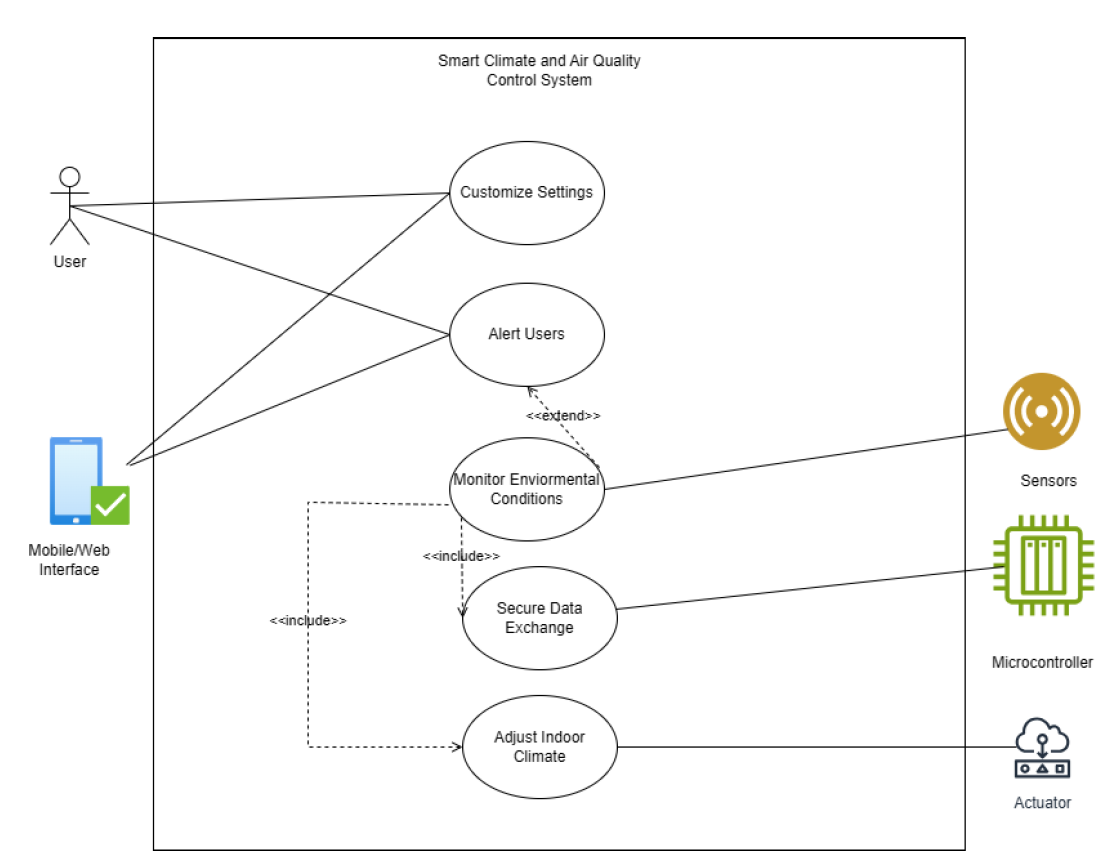
\includegraphics[width=\columnwidth]{images/UCD.png}
    \caption{Use Case Diagram}
    \label{fig:use_case}
\end{figure}

\section{System Overview and Operation}
The Smart Climate and Air Quality Control System is a comprehensive IoT-based solution designed to enhance indoor environmental quality through continuous monitoring and autonomous control. The key components include the PineCone1 microcontroller, a DHT22 sensor for temperature and humidity measurement, and specialized gas sensors for monitoring air pollutants. These components are interconnected to deliver real-time data processing, decision-making, and proactive control actions.

The system's architecture follows a modular and scalable design. Each sensor module communicates with the central microcontroller, which serves as the processing hub. The microcontroller is programmed in C to handle data acquisition, processing, and control logic. The MQTT protocol over Wi-Fi enables secure and efficient communication between the microcontroller and a data storage system, allowing remote access and management of environmental data.

The system operates continuously and performs several critical tasks autonomously:
\begin{itemize}
\item \textbf{Environmental Monitoring:} The sensors gather data on key parameters such as temperature, relative humidity and air quality metrics (e.g., CO concentration. Each sensor transmits real-time readings to the microcontroller.
\item \textbf{Data Processing and Analysis:} The microcontroller processes raw sensor data using programmed algorithms. Threshold-based decision-making algorithms compare current readings against predefined safety limits. In advanced implementations, machine learning models predict trends and identify patterns for more adaptive control.
\item \textbf{Automated Control Actions:} When environmental conditions deviate from the safe range, the system takes corrective actions. Examples include adjusting ventilation systems, activating air purifiers, or modifying thermostat settings. This ensures an optimal indoor environment with minimal user intervention.
\item \textbf{User Notifications and Interface:} Users interact with the system through a web interface. This dashboard displays live sensor readings. Customizable alerts notify users of critical conditions, providing proactive recommendations or manual control options.
\end{itemize}

\section{Challenges faced by the development team}
\textbf{Time Management} One of the primary difficulties was managing time effectively across different phases of the project. Multiple components, such as sensor integration, coding for microcontrollers, and developing the user interface, needed parallel attention. Synchronizing these tasks with a limited timeline created bottlenecks, particularly when debugging firmware issues took longer than anticipated.

\textbf{Resource Availability} Access to essential hardware components, such as sensors and microcontrollers, was occasionally delayed, affecting system testing timelines. This required contingency planning to focus on other project sections while waiting for physical resources.

\textbf{Debugging and Compatibility Issues} Integrating sensors like DHT22 sensors into the PineCone1 microcontroller posed compatibility challenges. Errors in sensor data readings and communication protocols using MQTT required extensive debugging, which slowed down progress.

\textbf{External Dependencies} The team had to continuously monitor service reliability and be prepared to switch or adapt solutions if needed.

\textbf{Documentation and Version Control} Maintaining up-to-date project documentation and managing version control for code was another recurring challenge. It was crucial to ensure that changes were logged properly to avoid confusion during collaborative development.

\begin{figure}[h] 
    \centering
    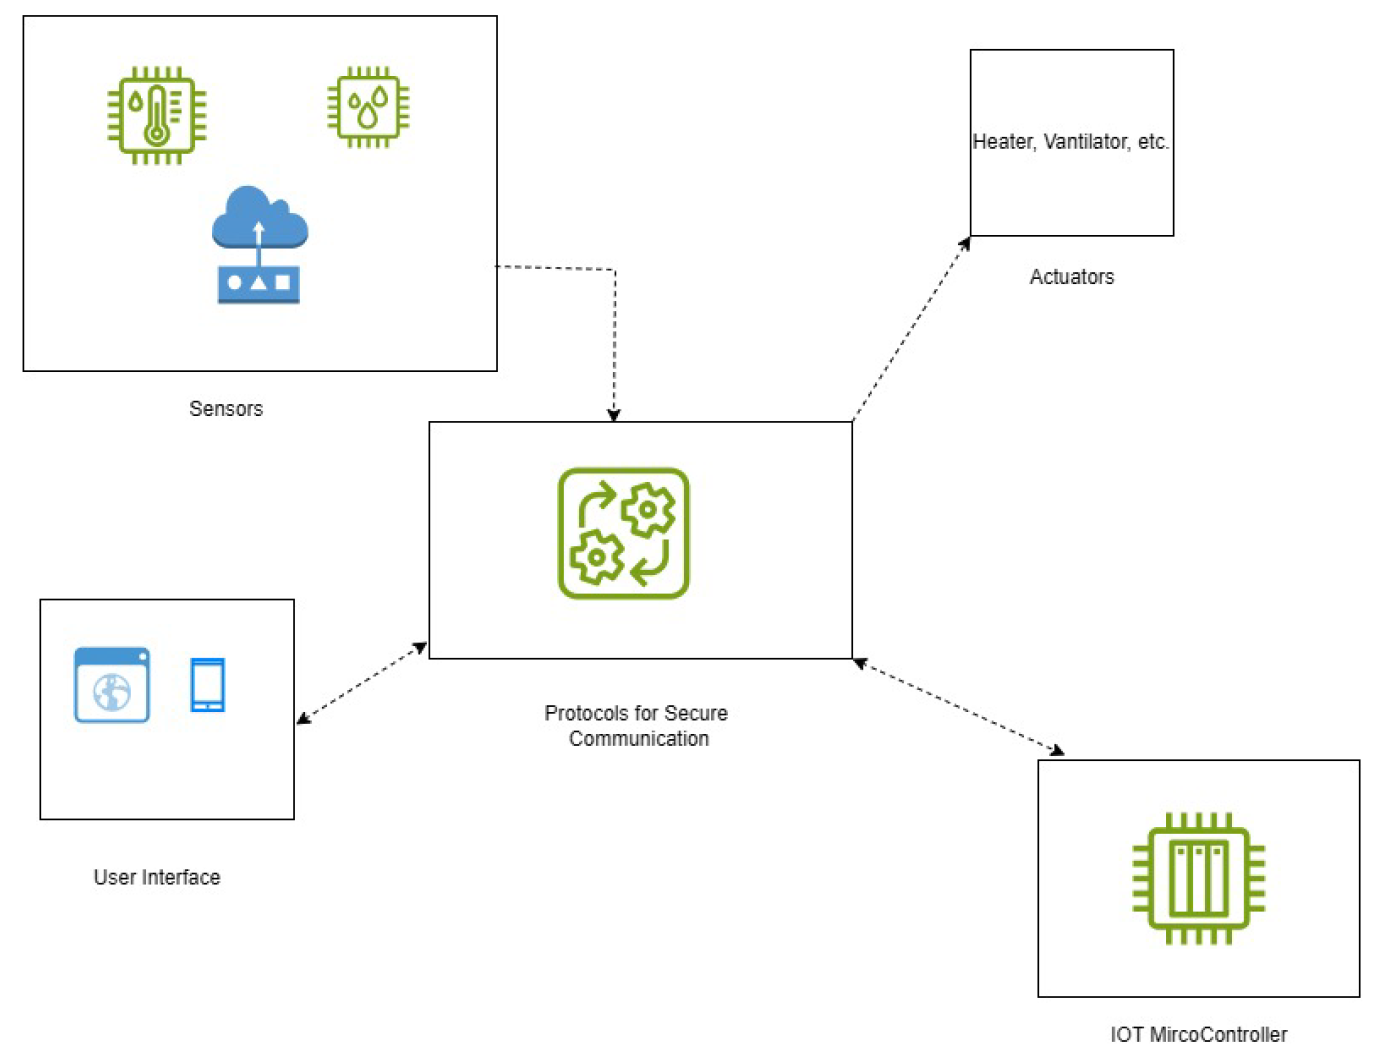
\includegraphics[width=\columnwidth]{images/AD.png}
    \caption{System Architecture}
    \label{fig:architecture}
\end{figure}

\section{Challenges and Limitations}
Developing an air quality control system for a smart home presents several technical and practical challenges. Sensor accuracy is a major concern, as low-cost sensors often suffer from calibration drift, requiring regular recalibration to maintain performance. Power consumption is another issue, especially in battery-operated systems, as continuous monitoring and operation demand energy efficiency. Connectivity and reliability also pose challenges, with IoT systems relying heavily on stable internet connections, which can be disrupted. Moreover, real-time data processing and decision-making require robust hardware and software to minimize latency. Integrating these systems with existing smart home ecosystems can be complex due to compatibility issues, while privacy and security concerns regarding sensitive data collection demand secure communication protocols, increasing development costs. Other limitations include high initial costs, environmental factors affecting sensor performance, and the need for regular maintenance to ensure long-term functionality. User experience is critical, as poorly designed interfaces can hinder adoption and effective use. Scalability is another concern, as systems must accommodate growing or changing household needs without significant reconfiguration. Additionally, regulatory compliance, limited market awareness, and challenges in implementing machine learning for predictive analytics can impede progress. Addressing these challenges requires balancing affordability, functionality, and user-friendliness while ensuring robust performance, security, and adaptability for long-term, sustainable use.

\section{Future Improvement}
Future improvements for air quality control systems will likely focus on enhancing sensor technology, enabling more accurate and reliable monitoring of pollutants, temperature, and humidity. Advancements in low-cost, high-precision sensors will reduce the need for frequent recalibrations and ensure consistent performance in diverse environments. Integrating advanced machine learning algorithms can enable predictive analytics, allowing systems to anticipate air quality issues and make proactive adjustments based on historical trends and real-time data. This capability would enhance energy efficiency and optimize resource usage, making these systems more sustainable and environmentally friendly. Additionally, hybrid systems combining natural ventilation with automated controls could further improve indoor air quality while reducing energy dependence. User experience will also see significant upgrades through more intuitive interfaces and customizable features. Mobile and web applications will likely evolve to provide users with actionable insights and detailed analytics, empowering them to take control of their indoor environment. Enhanced integration with smart home ecosystems and IoT platforms will make these systems more seamless and versatile, accommodating diverse user preferences and environmental conditions. Future designs will prioritize modularity, allowing for easy scalability and adaptation to various settings, from small apartments to large commercial spaces. Furthermore, robust data privacy and security measures, such as blockchain-based systems, will ensure user trust and compliance with evolving regulations. These improvements will collectively enhance the adoption and efficacy of air quality control systems, making healthier, smarter living environments a reality for more people.

\section{Conclusion}
Smart climate and air quality control systems represent a transformative leap in creating healthier, more efficient, and sustainable living environments. By integrating IoT technologies, advanced sensors, and automation, these systems optimize indoor conditions, reducing energy consumption and mitigating health risks associated with poor air quality and enhance life expectancy. Their ability to regulate temperature, humidity, and pollutants in real-time makes them indispensable for modern living, particularly in the face of climate challenges and rising energy costs. Furthermore, their applications extend beyond homes to schools, healthcare facilities, and smart cities, enhancing comfort, learning, and well-being in diverse settings. While challenges such as sensor calibration, data security, and high initial costs persist, ongoing advancements in sensor technology, machine learning, and modular design hold immense promise. Future improvements will focus on greater accuracy, predictive analytics, and seamless integration with smart ecosystems, ensuring these systems are more intuitive, scalable, and adaptable. By addressing these challenges and harnessing their full potential, smart climate and air quality control systems can lead to a sustainable future, where indoor spaces are not only comfortable but also environmentally conscious and health-promoting.

\printbibliography[title={References}]

\end{document}